\documentclass[t]{beamer}

\makeatletter
\let\th@plain\relax
\makeatother	

\usepackage{color}					%specify certain colors to configure e.g. hyperref
\usepackage[T1]{fontenc}			%german umlauts	
\usepackage[utf8]{inputenc}			%UTF-8 compatibility
\usepackage{graphics}
\usepackage{url}					%embeds URLs
\usepackage{marvosym}
\usepackage{media9}
\usepackage{listings}
%\usepackage{enumitem}
\usepackage{etoolbox}

\lstset{language=Python} 

\usepackage{color}

\definecolor{mygreen}{rgb}{0,0.6,0}
\definecolor{mygray}{rgb}{0.5,0.5,0.5}
\definecolor{mymauve}{rgb}{0.58,0,0.82}

\lstset{language=Python,
	basicstyle=\ttfamily,
	keywordstyle=\color{blue}\ttfamily,
	stringstyle=\color{red}\ttfamily,
	commentstyle=\color{green}\ttfamily,
	basicstyle=\tiny,
	breaklines=true,
	morecomment=[l][\color{magenta}]{\#}
}




\definecolor{hblue}{RGB}{51,51,178} %blue

	
\title[ORE]{Systemic Risk and the Open Source Risk Engine}
\author{Nikolai Nowaczyk}
\date{21/01/2017}

\usetheme{Boadilla}
%\usecolortheme{beaver}

\AtBeginSection[]
{
	\begin{frame}{Outline}
		\tableofcontents[currentsection,currentsubsection]
	\end{frame}
}

\beamertemplatenavigationsymbolsempty

\makeatletter
\patchcmd{\@listI}{\itemsep3\p@}{\itemsep1.2em}{}{}
\makeatother

\begin{document}

%\setlist[itemize]{itemsep=0.6em, label=$\blacksquare$}


\begin{frame}
	\maketitle
\end{frame}

\begin{frame}{Introduction}
	\begin{itemize}
		\item
		Nikolai Nowaczyk
		\begin{itemize}
			\item
				Consultant at Quaternion Risk Managment
			\item 
				currently staffed on projects in London
			\item
				2015-2016: Academic Visitor at Imperial College London			
			\item
				2011-2014: PhD in maths at Uni Regensburg			
			\item
				2005-2011: studied maths at Uni Bonn 
		\end{itemize}
		\item
			Quaternion Risk Managment
			\begin{itemize}
				\item
					Risk Managment company (consulting and software)
				\item
					offices in Dublin, London, New York and Düsseldorf
				\item
					core areas of expertise include Dynamic Initial Margin and CVA
				\item
					about 30 people and rapidly growing
			\end{itemize}
	\end{itemize}
\end{frame}
	
\begin{frame}{Key Points today}
	\begin{enumerate}
		\item
		A financial derivative is a contract between two counterparties that transfers a financial risk from one counterparty to another.
		\item
		The counterparties in a derivative trade are exposed to each others default risk.
		\item
		This risk can be drastically reduced by collateralizing the derivative trade.
		\item
		This reduction of risk comes at a significant cost - in money and overhead.	
		\item
		ORE is free and open source software that can be used to quantify and simulate the counterparty credit risk in derivatives trades.					
	\end{enumerate}
	
\end{frame}

\begin{frame}
	\tableofcontents
\end{frame}


\section{Financial Derivatives}


\subsection{FX risk: A practical example}

\begin{frame}{Case study: The great British bake off}
	\begin{itemize}
		\item
			Your grandmother from Yorkshire runs a small bakery business in the UK.
		\item
			The CEO of a large US firm is on holiday in Lake District and passes by your grandmother's bakery. 
		\item
			He is so impressed with the cake that he buys a huge order for his entire company and offers her \textbf{USD 1mn} to be paid on delivery in \textbf{1Y}.
		\item
			Granny has dreamed of running an international business for all her life and wants to enter into the deal.
			But when the runs the books, she realizes that she would first have to make an investment to expand the business so it can handle the big order. 
			This expansion would incur quite some costs first and of course she runs her business in \textbf{GBP}.
	\end{itemize}
	
	\begin{center}
		\textbf{Can she close the deal?}
	\end{center}
	
\end{frame}

\begin{frame}{A back of the envelope calculation (1)}
	\begin{itemize}
		\item 
			The current FX rate is $\mathbf{FX_{spot}=0.65}$, so \textbf{USD 1mn} is equal to \textbf{GBP 650k}.
		\item
			She needs to invest \textbf{GBP 550k} to deliver the order. That's a profit of \textbf{GBP 100k}.
		\item
			But then she studies the FX rate and realizes: The FX rate can change by about \textbf{15\%} over a year. If it moves into the wrong direction, she would only get \textbf{GBP 552.5k}. That is dangerously close to a loss!
		\item
			She doesn't want to loose this once-in-a-lifetime business opportunity, but she also doesn't want to risk her pension.			
	\end{itemize}
\end{frame}

\begin{frame}{A back of the envelope calculation (2)}
	\begin{center}
		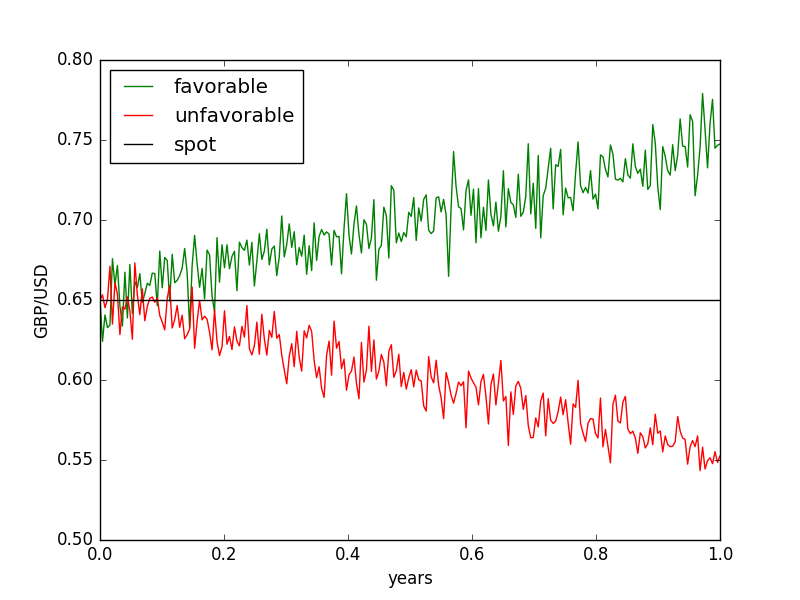
\includegraphics[scale=0.4]{pics/fx_scenarios.png}
	\end{center}
\end{frame}


\begin{frame}{FX Forward}
	\begin{definition}[FX Forward]
		An \emph{FX Forward} is a financial contract between two counterparties consisting of
		\begin{itemize}
			\item
				a \emph{domestic currency} (for instance GBP) and a \emph{foreign currency} (for instance USD),
			\item
				a \emph{notional} $N$ (for instance $N=1mn$ in foreign currency),
			\item
				a \emph{strike rate} $K$ (for instance $K=0.60$),
			\item
				a \emph{maturity} $T$ (for instance $T=1Y$),
		\end{itemize}
		which if incepted today at $t=0$ pays out 
			\begin{align*}
				N(K-FX_{T})
			\end{align*}
		at $t=T$ (in domestic currency), where $FX_T$ is the $FX$ rate at time $T$.
	\end{definition}
	Notice that although the FX Forward is bought today, the cashflow will happen in the future and can be positive or negative!	
\end{frame}

\begin{frame}{Hedging a future transaction}
	\begin{itemize}
		\item
			A cashflow at $T$ in the amount of $N$ in foreign currency will be worth $N \; FX_{T} $ in domestic currency, i.e. this cashflow is \emph{exposed} to an FX risk.
		\item
			A portfolio consisting of this future cashflow and an FX Forward with the same notional has a combined payoff of
			\begin{align*}
				N(K-FX_T)+N \; FX_T = N K
			\end{align*}
			and is completely determined today.
		\item
			In practice the strike $K$ of an FX Forward is often chosen in a way such that its current market price is $0$.
	\end{itemize}

	Assuming this strike is \textbf{K=0.6} and granny enters into the FX Forward at, she will have \textbf{GBP 600k} and therefore a profit of \textbf{GBP 50k} for sure!
	\begin{center}
		\textbf{Deal done!}
	\end{center}	
\end{frame}

\subsection{Terminology, Jargon, Basics}

\begin{frame}{Some comments, features and terminology}
	\begin{itemize}
		\item
			The FX Foward is a \emph{derivative}, the future cashflow is the \emph{underlying}, and the FX rate is the \emph{risk factor}.
		\item
			A derivative can be used to \emph{hedge} the \emph{market risk} in an \emph{underlying}. 
		\item
			A derivative works like an insurance against adverse market movements.
		\item
			A derivative may be bought without the underlying - for speculative reasons.
		\item
			The risk of changing future FX rates does not vanish via the derivative. It gets transferred from the buyer of the derivative (for instance a small business) to the issuer (for instance a big bank).
		\item
			A derivative like an FX Forward can in theory be created at any time and for any notional - it is not a ressource like gold. (In practice this creation requires quite some banking infrastructure though.)
	\end{itemize}
\end{frame}

\begin{frame}{Other products and features}
	\begin{itemize}
		\item
			An \emph{FX Option} is a derivative similar to an FX Forward, but the payoff is $N(K-FX_{T})^{+} \geq 0$ (that one always costs a premium to buy).
		\item
			There are many more derivatives, but a common theme is that something is agreed on in advance and that something is either mandatory (Forward) or optional (Option).
		\item
			There are many more asset classes that have derivatives: 
			\begin{itemize}
				\item
					IR (Interest Rates)
				\item
					FX (Foreign Exchange)
				\item
					CDS (Credit Default Swap)
				\item
					EQ (Equities)
				\item
					CO (Commodities).
			\end{itemize}
		\item
		Derivatives are financial goods themselves and can be traded. As a result their prices change just like the underlyings.			
	\end{itemize}
\end{frame}

\begin{frame}{Summary}
	\begin{itemize}
		\item
			A financial derivative is a contract between two counterparties that transfers a financial risk from one counterparty to another.
		\item
			Derivatives themselves are traded and change in value.
	\end{itemize}
\end{frame}

\section{Counterparty Credit Risk (CCR)}

\subsection{The problem of ''too big to fail''}

\begin{frame}{Coming back to our example: Good old times}
	\begin{itemize}
		\item
			Granny has closed the deal. Everything goes well. The FX rate dropped by 15\%, so she is really happy about the FX Forward, which is now worth a lot of money.
	\end{itemize}
	\begin{center}
		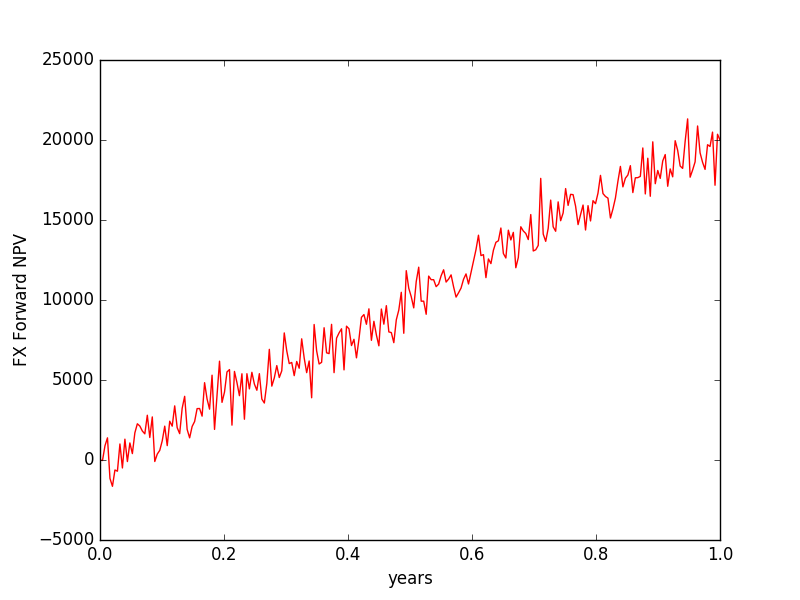
\includegraphics[scale=0.4]{pics/fx_foward_rising.png}
	\end{center}		
\end{frame}

\begin{frame}{Coming back to our example: Financial crisis}
	\begin{itemize}
		\item
			Suddenly she reads in the news that the bank she bought the Forward from went bust.
		\item
			The bank failure causes a major market turmoil and the FX rate goes down another 10\%.
		\item
			When she receives the USD transaction, the GBP equivalent is not nearly enough to cover her costs. She suffers a huge loss and her business goes bust too.
	\end{itemize}
	\vspace{-2em}
	\begin{center}
		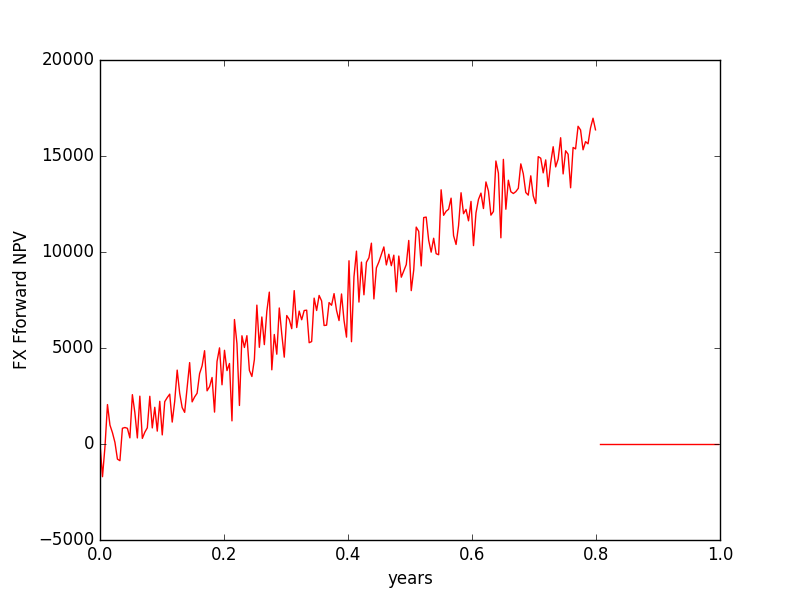
\includegraphics[scale=0.25]{pics/fx_default.png}
	\end{center}		
\end{frame}


\begin{frame}{Derivatives and CCR}
	\begin{itemize}
		\item
			\emph{Counterparty Credit Risk} is the risk that a counterparty does not satisfy its contractual obligations to you, because it goes bankrupt before the end of the contract.
	\item
		CCR has a long history in finance, in particular in credit! Loans are the oldest example where this risk component is very well encorporated into the business.
	\item
		During the crisis in 2007/08 people realized that derivatives have a credit risk component too. A derivative issued by a bank that goes bust is worth nothing.
	\item
		Since derivatives transfer risk from one counterparty to another, a bank failure transfers it back in an unpredictable way, which has a knock-on effect.
	\end{itemize}
\end{frame}

\begin{frame}{What has happened since the crisis}
	\begin{itemize}
	\item
		People realized that certain banks and financial institutions are \emph{too big to fail}, i.e. their failure would cause knock-on effects on other banks that are so disastrous that they would fail too. This chain reaction endangers the world's finance system as a whole, hence the term \emph{systemic risk}.
	\item
		If such an institution would crumble, the government could save it using tax payers money (hugely unpopular).
	\item
		Tighter regulation, higher capital requirements and stress testing have been introduced.
	\end{itemize}

	\begin{center}
		\textbf{The rules of the game for derivative trading have changed to mitigate counterparty credit risk via the introduction of \emph{margining}!}
	\end{center}
\end{frame}

\subsection{Collateralization of Derivative Trades}

\begin{frame}{Uncollateralized derivative trades}
	\begin{itemize}
		\item
			``Old world'' style of trading.
		\item 
			Payments between counterparties are only exchanged at the payment dates (for the FX Forward only at inception and maturity). 
		\item
			Between those dates, the counterparties are fully exposed to each other's credit risk.
	\end{itemize}
	\vspace{-2em}
	\begin{center}
		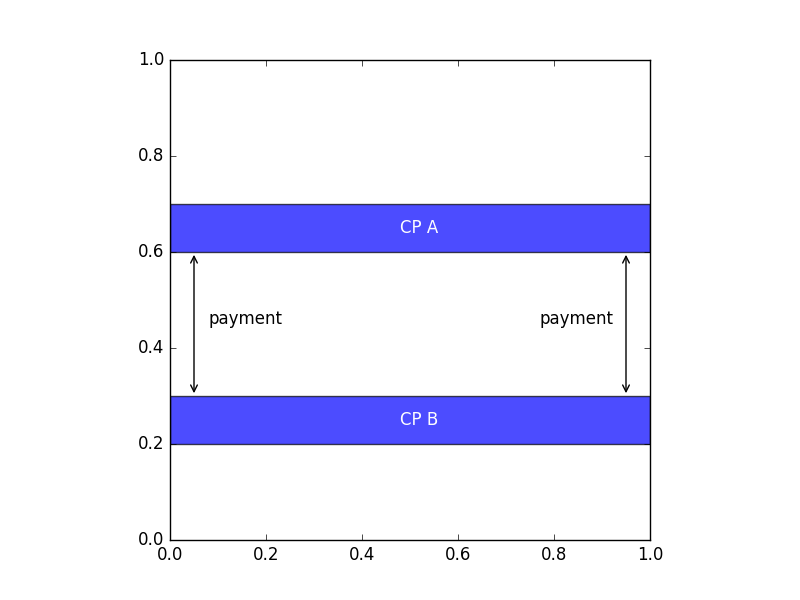
\includegraphics[scale=0.35]{pics/cashflows_uncoll.png}
	\end{center}	
\end{frame}

\begin{frame}{VM collateralized trades}
	\begin{itemize}
		\item
			At inception CPs A and B exchange payments.
		\item
			The day after, the value of the derivative has changed by some $\Delta$. If this is positive for $A$, then $A$ pays $\Delta$ to $B$. If it is negative $B$ pays $\Delta$ to $A$. These payments are called \emph{variation margin} (VM).
		\item
			This procedure is repeated \underline{every day} after inception till maturity.
	\end{itemize}
	\vspace{-2em}
	\begin{center}
		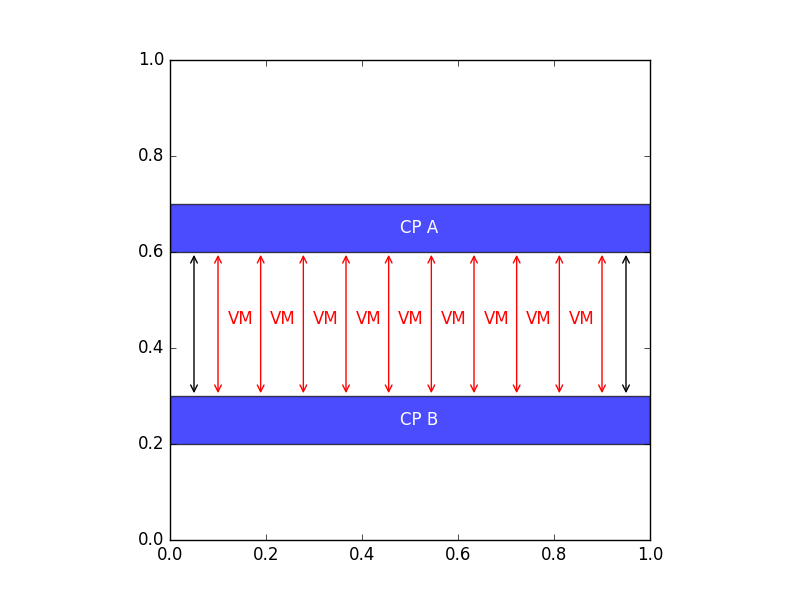
\includegraphics[scale=0.35]{pics/cashflows_vm_coll.png}
	\end{center}	
\end{frame}

\begin{frame}{Features of a VM collateralized derivative trade}
	\begin{itemize}
		\item
			The sum of all payments exchanged in an uncollateralized trade is the same as the sum of all payments exchanged in the VM collateralized trade.
		\item
			Both CPs are no longer exposed to each others credit risk assuming:
		\begin{itemize}
			\item
				Defaults only happen instantanously after VM payments.
			\item
				CPs notify each other instantanously after a default.
			\item
				The surviving CP is able to instantanously buy the exact trade it has lost from another CP for exactly the amount of VM it has collected.
		\end{itemize}
	\end{itemize}
	\begin{center}
		\textbf{In reality, none of these assumptions is satisfied!}
	\end{center}
\end{frame}

\subsection{(Dynamic) Initial Margin}

\begin{frame}{The MPOR}
	\begin{itemize}
		\item
			In reality there is a gap between the \emph{default date} and the \emph{close out date}, i.e. the date at which the surviving counterparty has been able to replace all trades from the defaulting counterparty with trades with some other counterparty.
		\item
			This gap is called the MPOR (Margin Period of Risk) and in practice is assumed to be between 5d to 20d.	
	\end{itemize}
	\vspace{-1em}
	\begin{center}
		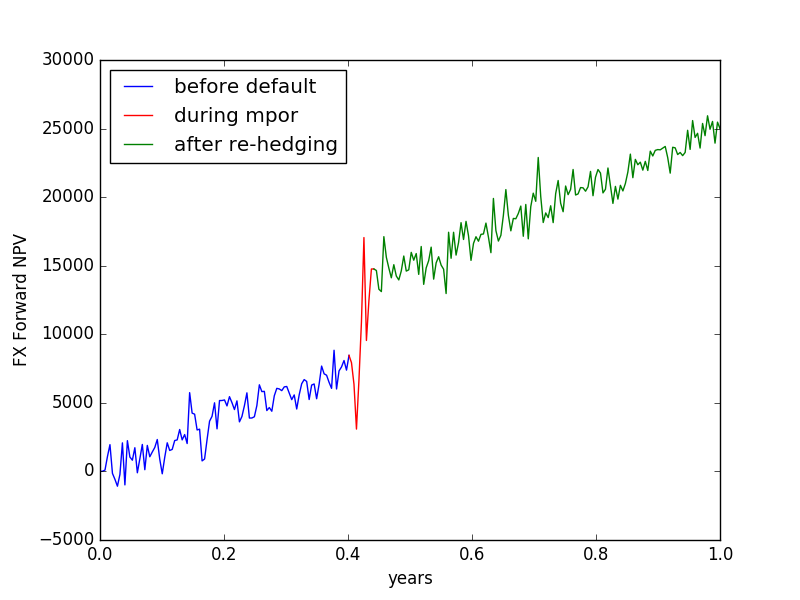
\includegraphics[scale=0.35]{pics/mpor_gap.png}
	\end{center}
\end{frame}

\begin{frame}{The role of Initial Margin}
	\begin{itemize}
		\item
			It is assumed that during the MPOR the markets will be in an extremely stressed regime, since the default of a major bank will cause an enormous turmoil. 
		\item
			At worst the markets will move massively against the surviving CPs favor still resulting in a big loss, since the received VM does not suffice to replace the trades at the closeout date.
	\end{itemize}
	\begin{center}
		\textbf{Solution: Banks have to post \emph{Initial Margin} (IM) in addition to VM to each other to cover for potential losses during the MPOR.}
	\end{center}
\end{frame}

\begin{frame}{Cashflows in a VM \& IM collateralized trade}
	\begin{center}
		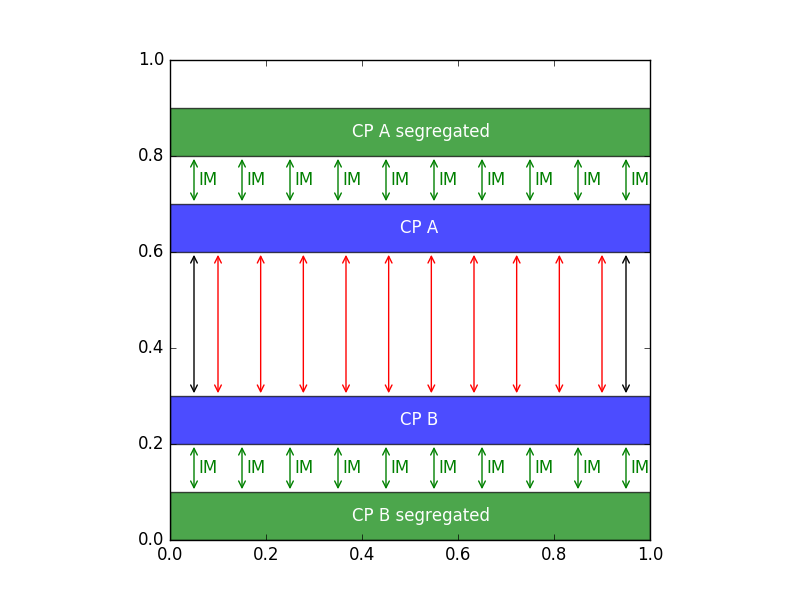
\includegraphics[scale=0.4]{pics/cashflows_im_vm_coll.png}

		\textbf{The administrative overhead of trading VM and IM collateralized derivatives is much higher for secured trades than for uncollateralized trades.}
	\end{center}
\end{frame}

\begin{frame}{Features of a VM \& IM collateralized trade}
	\begin{itemize}
		\item
			The overall CCR in derivatives trading is reduced drastically.
		\item
			VM may be \emph{rehypothicated}, i.e. you may use the VM you received from CP A to post your VM to CP B. IM may not be rehypothicated, which makes this very expensive.
		\item
			Pricing an uncollateralized derivative and simulating its future value is already a very complex modelling challange and considered as the holy grail of mathematical finance.
		\item
			The overwhelming majority of literature on derivative pricing does not (yet) account for VM and IM and therefore, most of these models do no longer reflect the reality of trading.
	\end{itemize}
\end{frame}

\begin{frame}{Dynamic Initial Margin}
	\begin{itemize}
		\item
			The term \emph{Initial Margin} is misleading: At inception it is paid initially based on a model and the current market conditions.
		\item
			If the market conditions change after the initial Initial Margin is posted and before the trade matures, a \emph{margin call} is initiated to re-adjust the IM based on the updated market conditions.
		\item
			Therefore, the introduction of Initial Margin, which was designed to mitigate risk, actually introduces a new risk. 
		\item
			In presence of IM banks need to plan ahead for future margin calls. 
		\item
			This planning ahead is called DIM (Dynamic Initial Margin) and is one of Quaternions' core business areas.
	\end{itemize}
\end{frame}

\begin{frame}{With one notable exception...}
	\begin{center}
		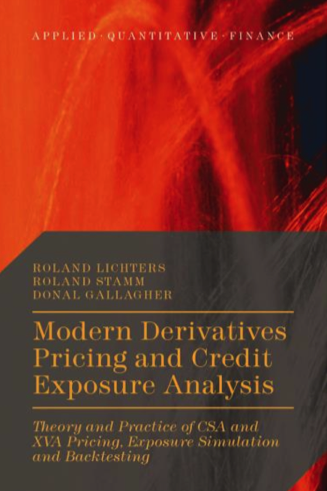
\includegraphics[scale=0.5]{pics/book.png}
	\end{center}
\end{frame}

\begin{frame}{Summary}
	\begin{itemize}
		\item
			The counterparties in a derivative trade are exposed to each others default risk.
		\item
			This risk can be drastically reduced by collateralizing the derivative trade.
		\item
			This reduction of risk comes at a significant cost - in money and overhead.
	\end{itemize}
\end{frame}

\section{Open Source Risk Engine}

\subsection{The technical side}

\begin{frame}{Risk Managment Systems}
	Banks have had risk managment systems for decades. These systems are
	\begin{itemize}
		\item
			massive! They typically involve 
			\begin{itemize}
				\item 
					large databank systems to store information about clients, trades and the markets.
				\item
					computer clusters to perform a massive amount of computations in parallel.
				\item
					complex reporting systems.
				\item
					many desktop clients to be used by the banks staff.
			\end{itemize}
		\item
			top secret, proprietary, closed source and a mixture of bought black-box software and in-house developments.
		\item
			constantly in need of updating, maintainance, bugfixing, refurbishment, extension etc.
		\item
			\textbf{intransparent}.
	\end{itemize}
\end{frame}

\begin{frame}{Practical problems}
	\begin{itemize}
		\item
			If such a risk managment system computes some number that sounds reasonable, how can we be sure it is actually correct? (\textbf{validation})
		\item
			If bank A issues a margin call to bank B based on their risk managment system and bank B claims that according to their system bank A is not right about this, what can they do? (\textbf{Margin dispute})
		\item
			How can a regulator know what a bank is actually calculating and how can a bank explain its reported numbers? (\textbf{control}) 
		\item
			How can the regulator make sure two banks with comparable trades are actually treated comparably? (\textbf{fairness in competition})
	\end{itemize}
\end{frame}

\subsection{Purpose of ORE}

\begin{frame}{Open Source Risk Engine}
	\begin{itemize}
		\item
			ORE is a free and open source software that can perform complex risk managment computations like a production system in a bank.
		\item
			Based on QuantLib - a free and open source library for pricing derivatives.
		\item
			Developed and released on github by Quaternion Risk Managment.  
		\item
			Its purpose is to
				\begin{itemize}
					\item
						serve as an independent reference implementation of risk.
					\item
						be useful for banks to validate an implementation of a model.
					\item
						be serious about transparency in banking.
					\item
						better connect academics and practitioners.
					\item
						inspire new ideas on what can be done with open source software in finance.
				\end{itemize}
	\end{itemize}
\end{frame}

\subsection{What ORE does}

\begin{frame}{What does ORE compute?}
	ORE computes the \emph{collateralized exposure}
	\begin{align*}
	EPE(t) := (V(t) - VM(t) - IM(t) )^+
	\end{align*}
	of a derivatives portfolio (among other things, greatly simplified). Here
	\begin{itemize}
			\item
				$V(t)$ is the simulated value of the portfolio at time $t$,
			\item
				$VM(t)$ is the simulated VM collateral at time $t$,
			\item
				$IM(t)$ is the simulated IM collateral at time $t$ and
			\item
				$EPE(t)$ is the \emph{expected positive exposure} at time $t$. 
	\end{itemize}
	The $EPE(t)$ is the amount of money you would lose if the counterparty defaults at $t$. It is a quantitative measure of the counterparty credit risk.
\end{frame}

%\begin{frame}{What does ORE compute?}
%	ORE has a complex input, which includes:
%	\begin{itemize}
%		\item 
%			The portfolio data, which defines all the trades to be analyzed.
%		\item
%			A grid of future dates on which to simulate.
%		\item
%			A number of Monte Carlo Paths.
%		\item
%			Auxiliary data like market data, conventions, details of the simulation etc. 
%	\end{itemize}
%	ORE produces several output files, in particular an \textbf{NPV cube}, i.e. a 3D array that for each trade, date and sample, stores the value of that trade in that sample at that date.
%	\begin{center}
%	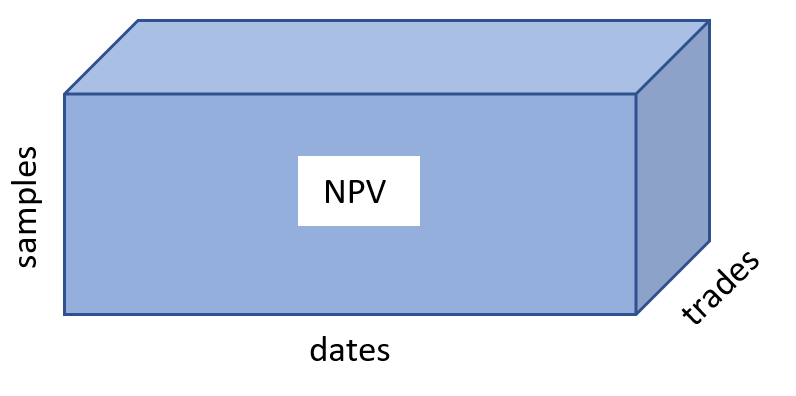
\includegraphics[scale=0.5]{pics/npv_cube_scheme.png}
%\end{center}
%\end{frame}

\begin{frame}{ORE Data Flow}
	\begin{center}
		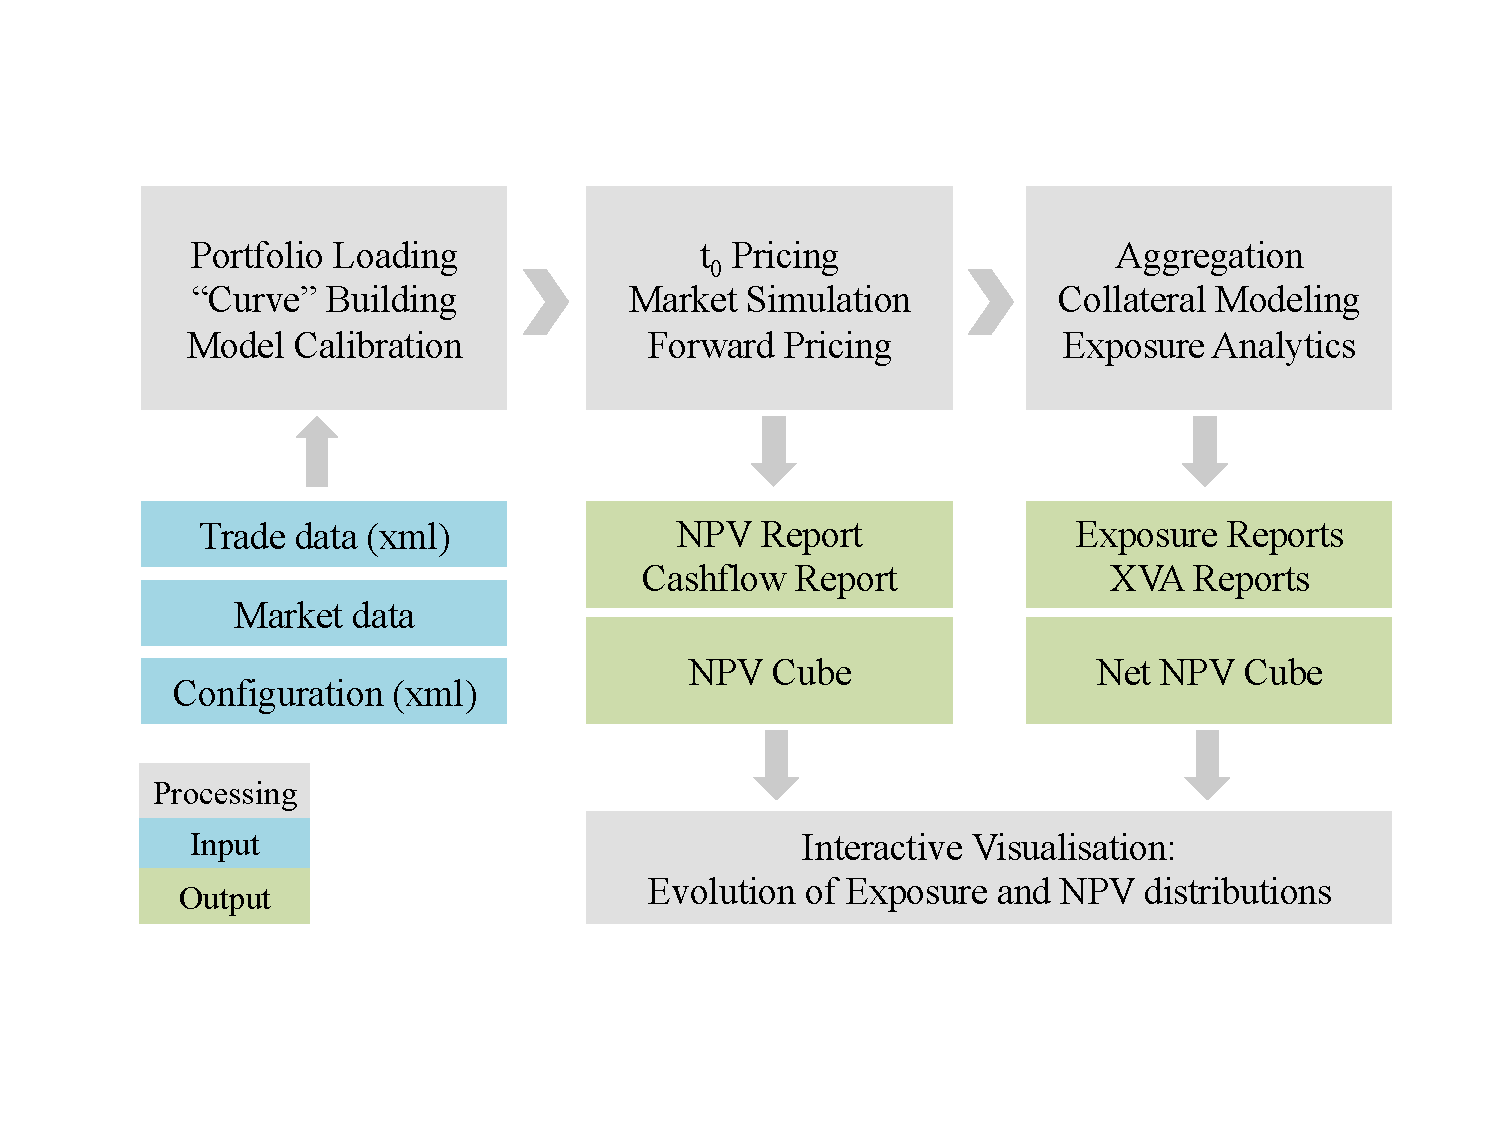
\includegraphics[scale=0.5]{pics/ore_process.pdf}
	\end{center}
\end{frame}

\begin{frame}{Trade Portfolio XML Input}
	\begin{center}
		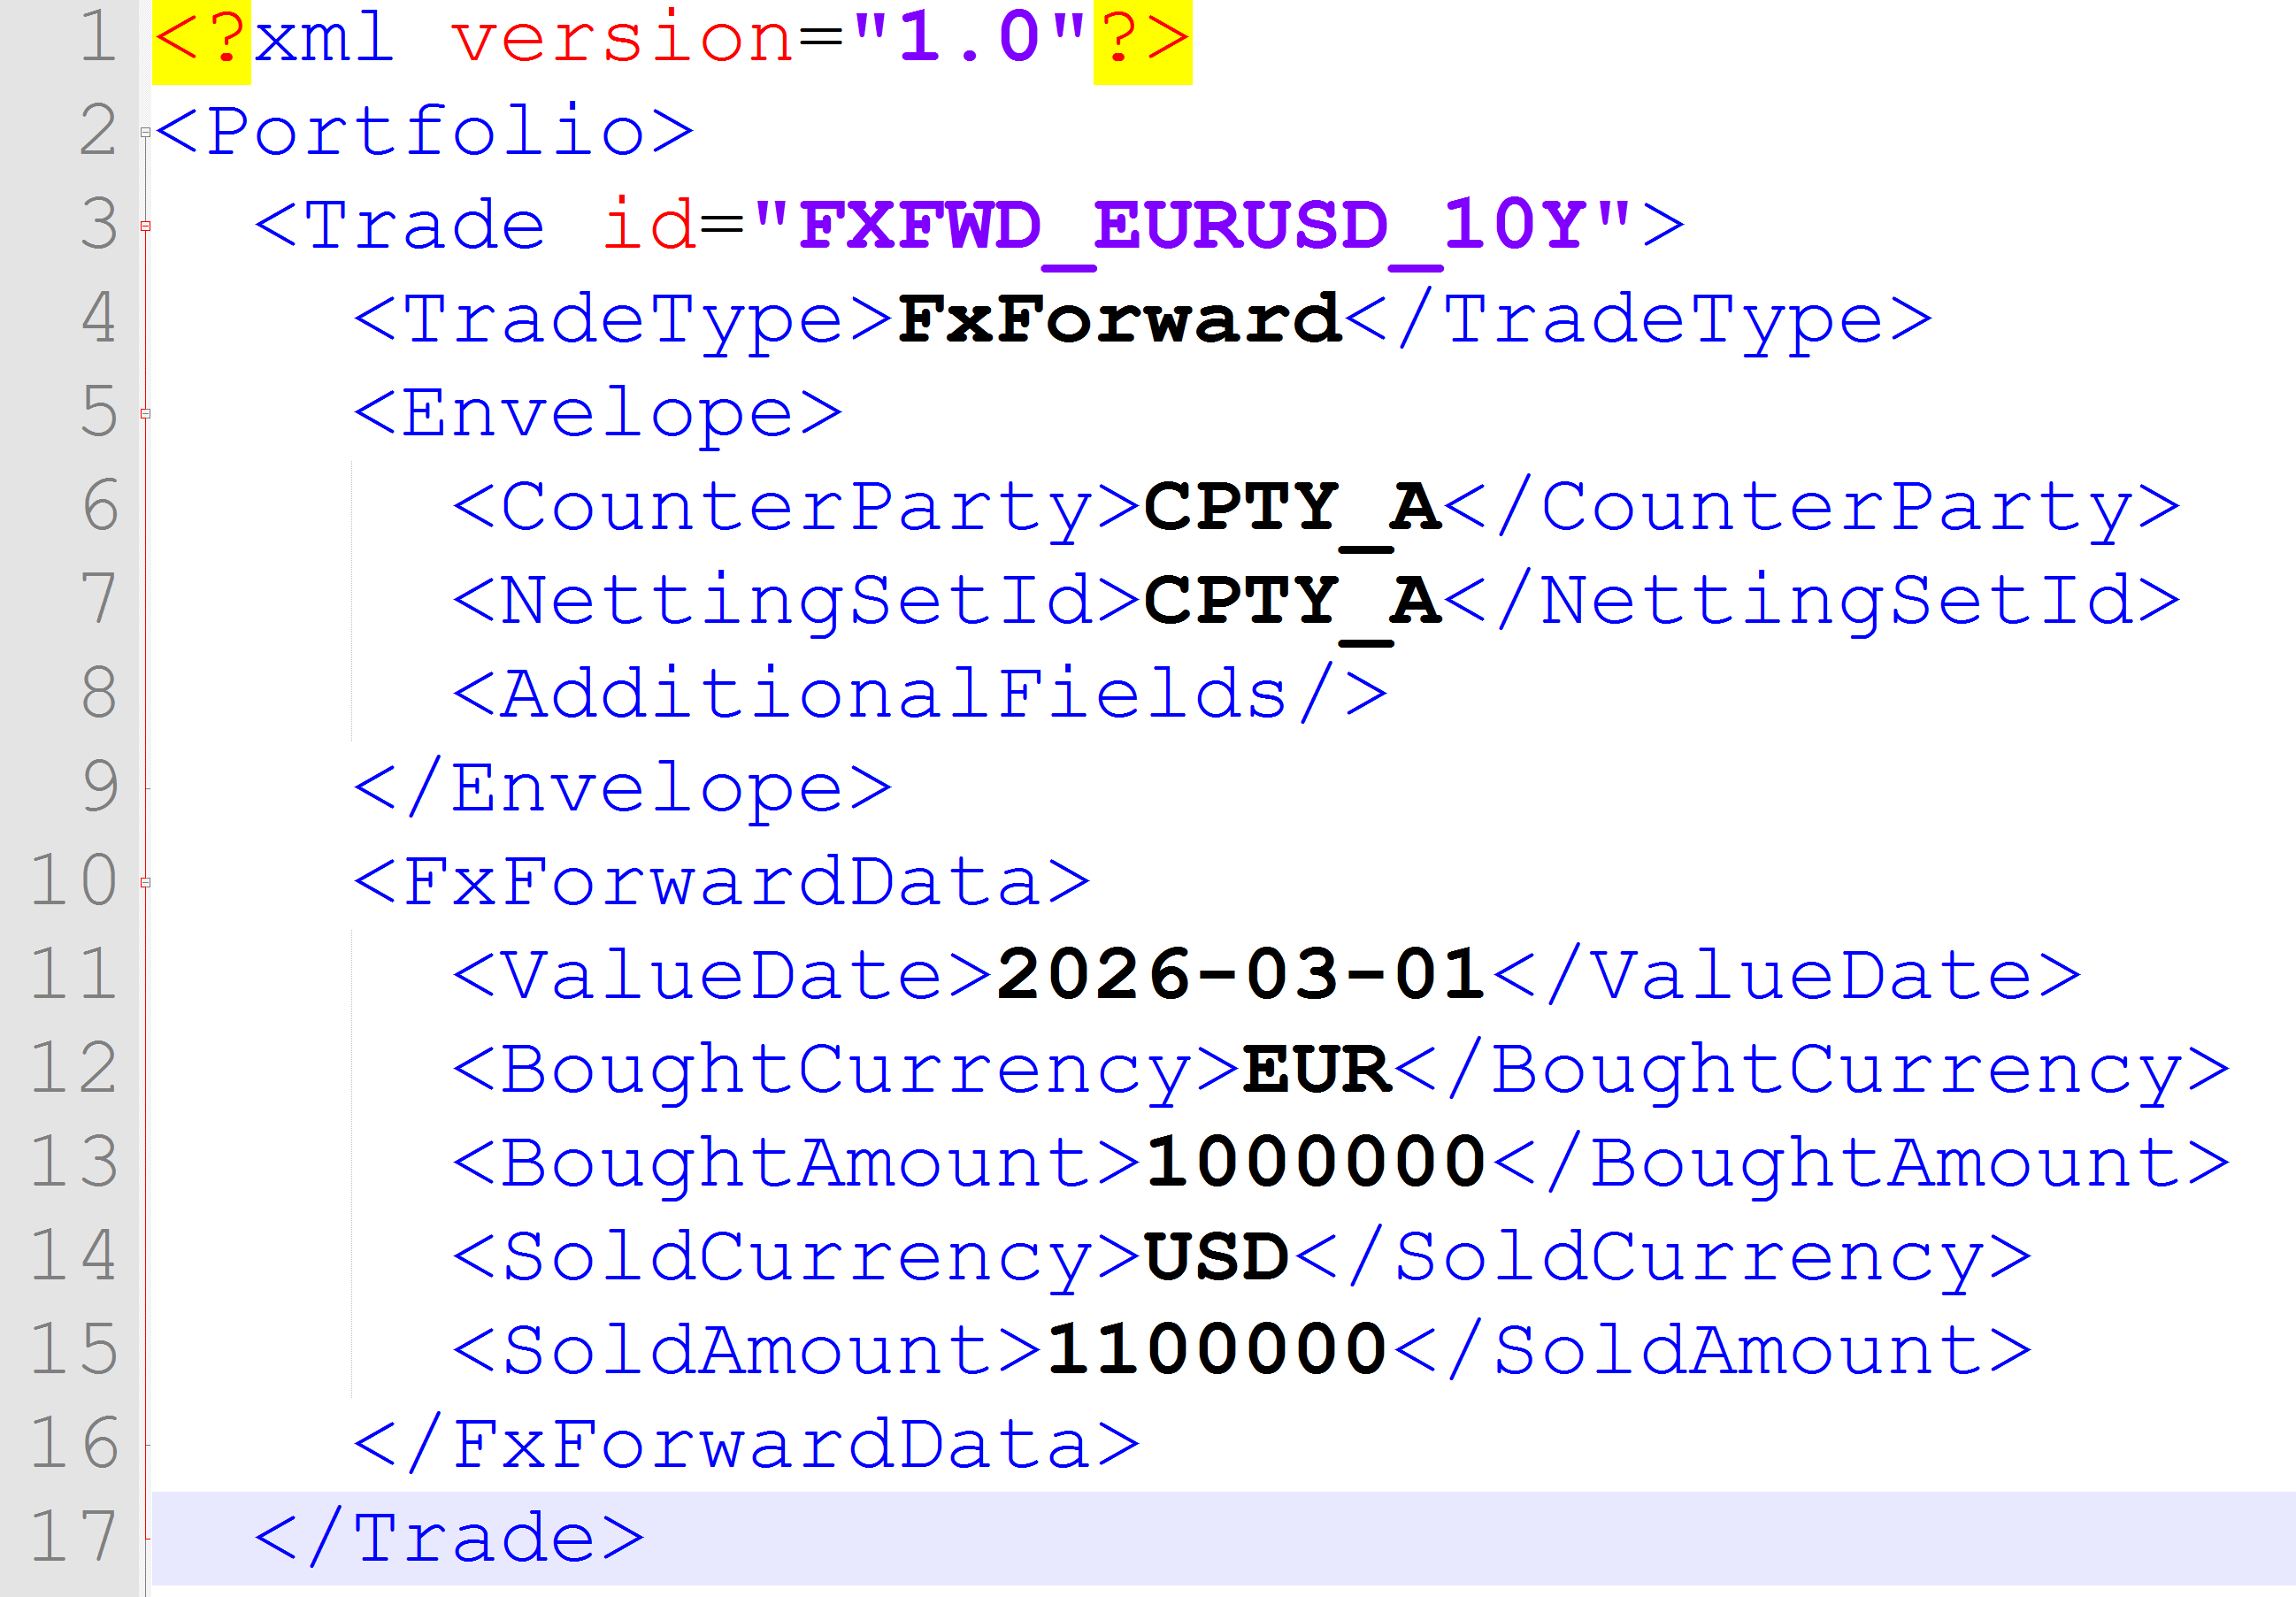
\includegraphics[scale=0.4]{pics/input_xml.png}
	\end{center}
\end{frame}

\begin{frame}{Kicking off a run}
	\begin{center}
		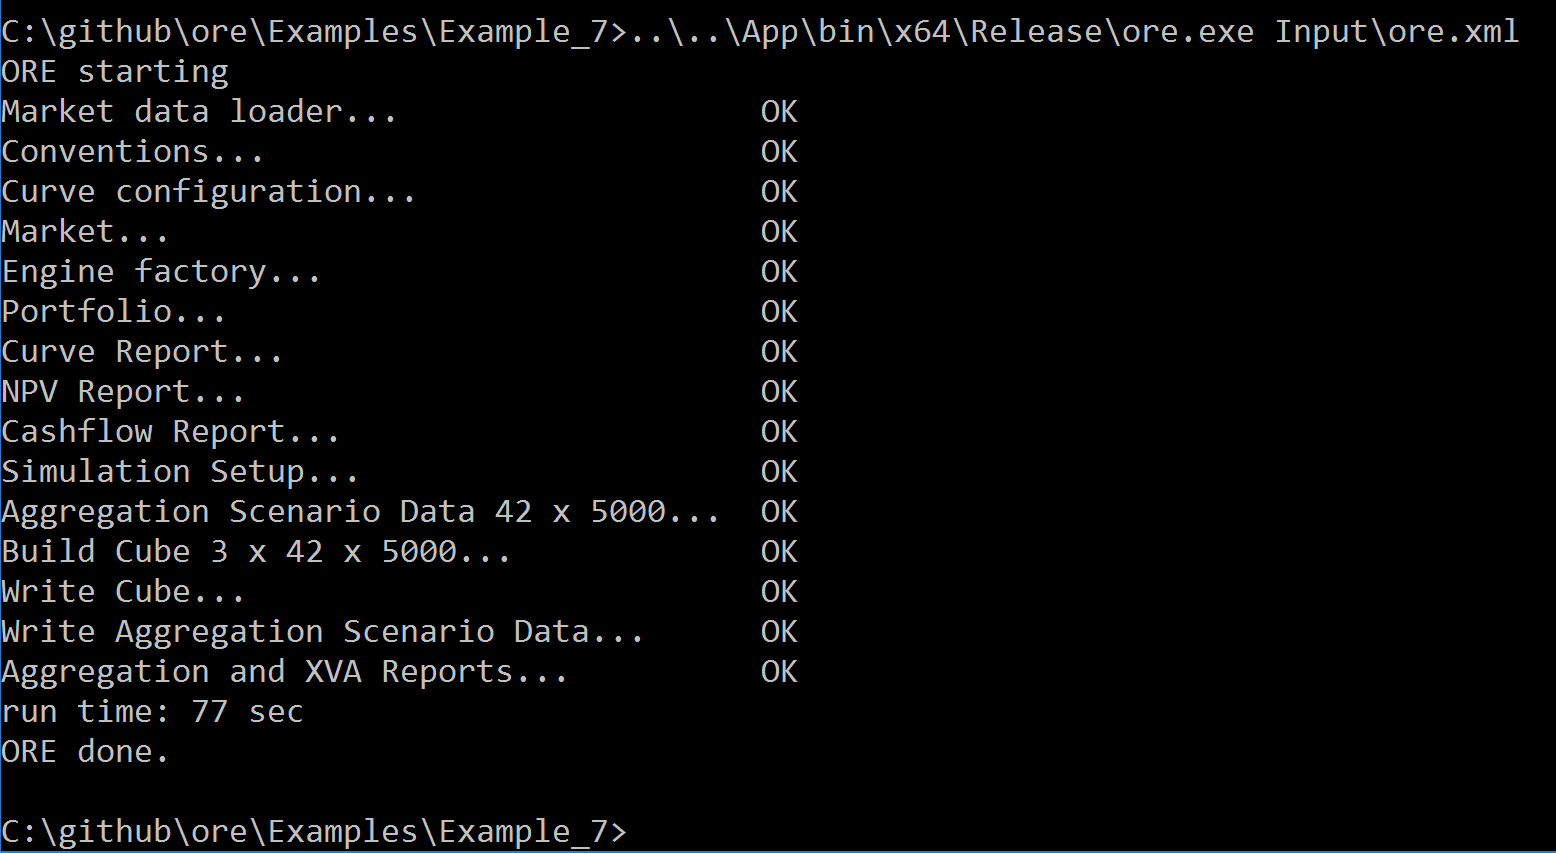
\includegraphics[scale=0.7]{pics/ore_console_run.png}
	\end{center}
\end{frame}


\begin{frame}{NPV Cube as a CSV Output}
	\begin{center}
		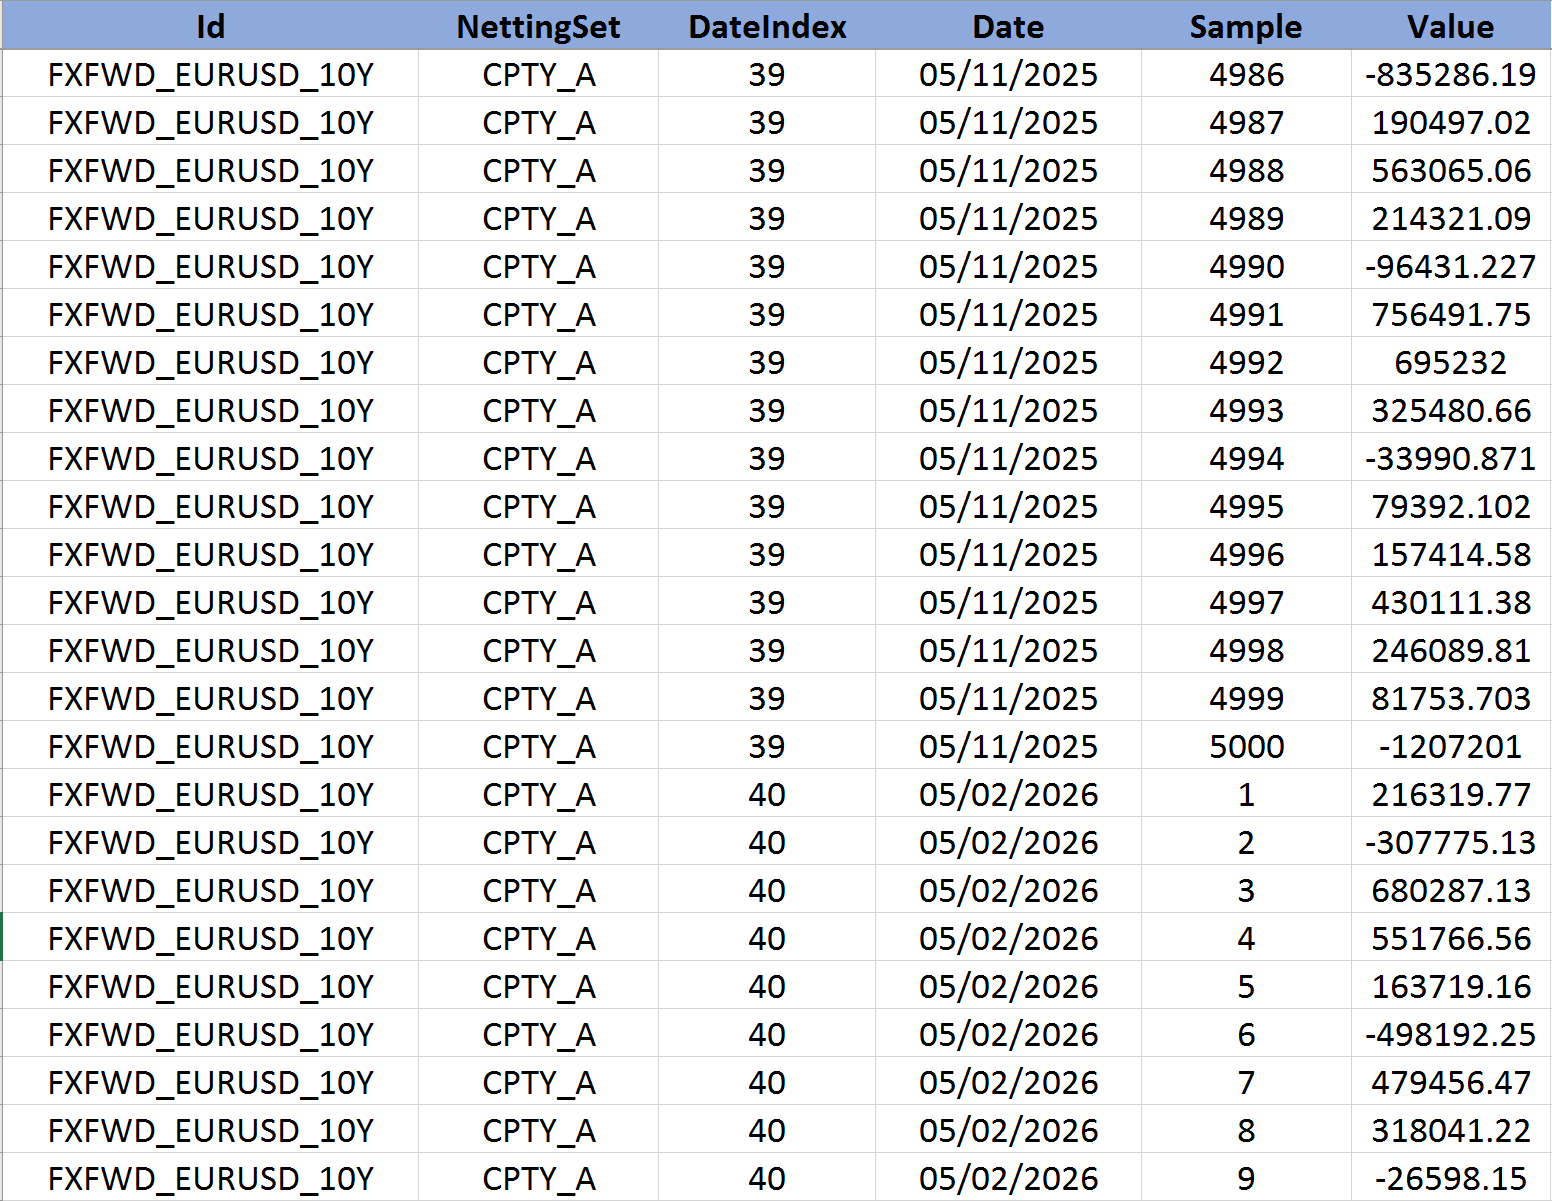
\includegraphics[scale=0.55]{pics/ore_csv_npv_cube.png}
	\end{center}
\end{frame}

\begin{frame}{Exposure Metrics}
	\begin{center}
		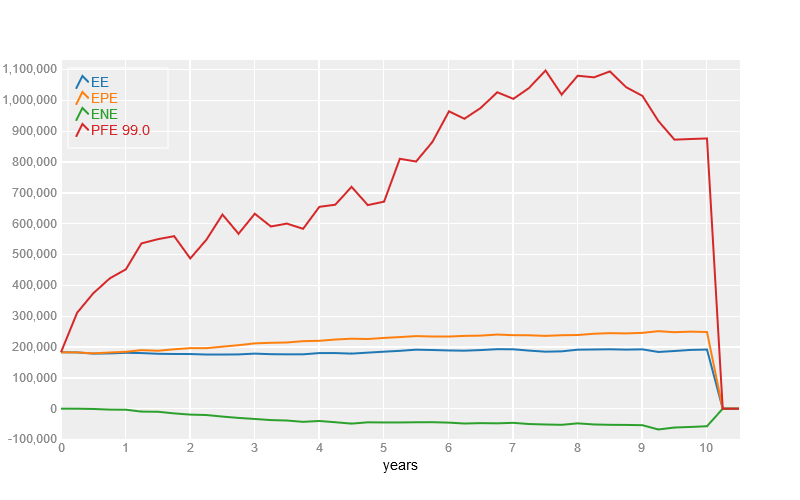
\includegraphics[scale=0.4]{pics/bqp_exposure_metrics.png}
	\end{center}
\end{frame}

\begin{frame}{Exposure Surface}
	\begin{center}
		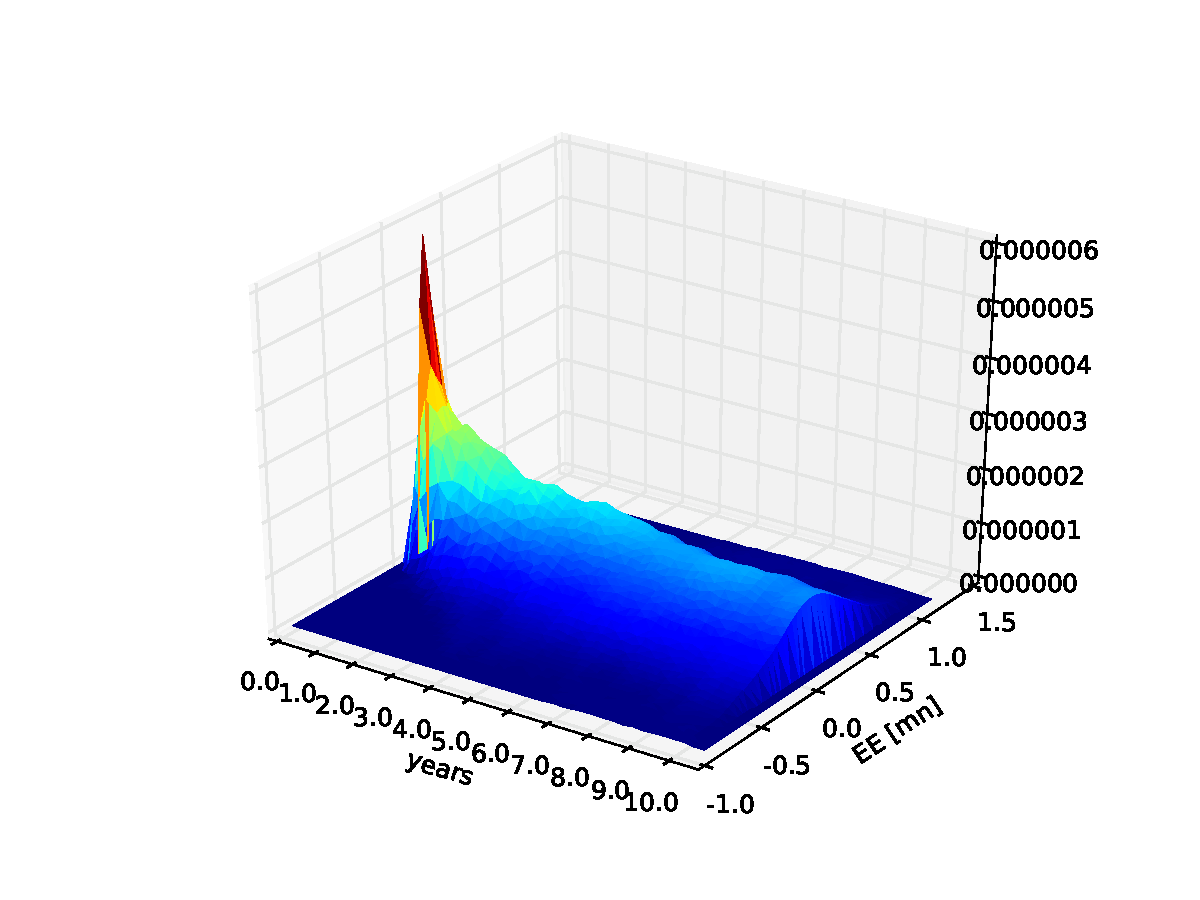
\includegraphics[scale=0.5]{pics/mpl_exposure_surface.pdf}
	\end{center}
\end{frame}

\begin{frame}{Summary}
	\begin{itemize}
		\item
			Risk managment systems of banks are inaccessible to academics.
		\item
			ORE is free and open source and a realistic simulation of a banks risk managment system.
		\item
			ORE can be used to quantify and simulate the counterparty credit risk in derivatives trades.
	\end{itemize}
\end{frame}

\section{A vision for the Capstone project}

\begin{frame}{A vision for this project}
	ORE provides a unique opportunity for a collaboration between academia and practice. We are among the first group of people with access to a free and open source software that realistically simulates a bank in (almost) all its complexities (ORE and QuantLib have about 400k lines of C++ code).
	\begin{itemize}
		\item
			Learn how to use ORE to simulate a trade, a portfolio, a bank.
			\begin{itemize}
				\item 
					Start with the examples supplied with ORE.
				\item
					Modify these examples and play around with them.
				\item
					(Define your own examples.)
			\end{itemize}	
		\item
			Coding project: Simulate a consortium of banks and study quantitatively the systemic risk in that system.
			\begin{itemize}
				\item
					Define a toy problem to study systemic risk using ORE. 
				\item
					Define portfolios for a handful of banks (2-5) and run all their portfolios through ORE.
				\item
					Develop a systemic risk dashboard that visualizes the systemic risk.
			\end{itemize}
	\end{itemize}
\end{frame}

\begin{frame}{Further Deliverables}
	\begin{itemize}
		\item
			Use these tools to write a project report that studies systemic risk based on the quantitative evidence gathered via the coding project. More concretely, the following points could be addressed:
			\begin{itemize}
					\item 
						Define exposure metrics for a single counterparty in that system. Define exposure metrics for a system of counterparties. 
					\item
						Summarize existing measures of systemic risk (as described for instance in \emph{Systemic Risk, Crises, and Macroprudential Regulation by Freixas et al.}) Define alternative measures of systemic risk as found in the literature and explore the strengths, opportunities and robustness of these measures.
				\item
					What is the total Initial Margin that is posted in that system? How does the total Initial Margin in the system change over time? (Think about the interplay between Initial Margin and Liquidity.) Can one reduce the Initial Margin in the system without substantially increasing the risk in the system?
			\end{itemize}	
		\item
			Write a summary of the project report that can be published as a paper.
	\end{itemize}
\end{frame}



\end{document}


